\chapter{Apprendimento non supervisionato: K-means e SOM}\label{ch-19}

Questa lezione è un'introduzione leggera all'\textbf{apprendimento non
supervisionato} con le reti neurali. Il fuoco è sul \textbf{clustering}
visto come \textbf{quantizzazione vettoriale}: si parte dal classico
\textbf{K-means} e si arriva a un modello neurale storico, le
\textbf{Self-Organizing Map} (SOM) di Kohonen, che aggiungono al
clustering la proprietà di preservare la topologia e quindi di
visualizzare i dati.

\section{Apprendimento non
supervisionato}\label{apprendimento-non-supervisionato}

Nell'apprendimento \textbf{non supervisionato non c'è insegnante}: il
training set contiene solo dati \textbf{non etichettati}
\(\langle \mathbf{x}\rangle\). I task principali:

\begin{itemize}
\tightlist
\item
  \textbf{Clustering}: trovare raggruppamenti naturali nei dati.
\item
  \textbf{Riduzione di dimensionalità}, visualizzazione,
  pre-elaborazione: i dati multidimensionali vengono proiettati in uno
  spazio a dimensione minore (PCA, Multi-Dimensional Scaling,
  Independent Component Analysis\ldots).
\item
  Modellazione della densità dei dati (non trattata nel corso).
\end{itemize}

A cosa serve? Esempi: organizzare le forme di vita in una tassonomia
(cosa sono i mammiferi?); i neonati imparano a riconoscere (a
``raggruppare'') i volti familiari prima di capire il linguaggio.
Soprattutto, i \textbf{dati non etichettati costano molto meno}: ad
esempio 10 milioni di frame di YouTube hanno permesso risultati allo
stato dell'arte nel riconoscimento di oggetti in 22.000 categorie.

\subsection{Clustering}\label{clustering}

\begin{boxdefinition}{Clustering}

Partizionare i dati in \textbf{cluster} (sottoinsiemi di dati
``simili''): i pattern di un cluster sono più simili tra loro che a un
pattern di un altro cluster. Ogni cluster è rappresentato da un
\textbf{centroide} (detto anche prototipo, vettore di riferimento,
centro del cluster, \emph{codevector}; l'insieme dei centroidi è il
\textbf{codebook}).

\end{boxdefinition}

\begin{figure}[htbp]
\centering
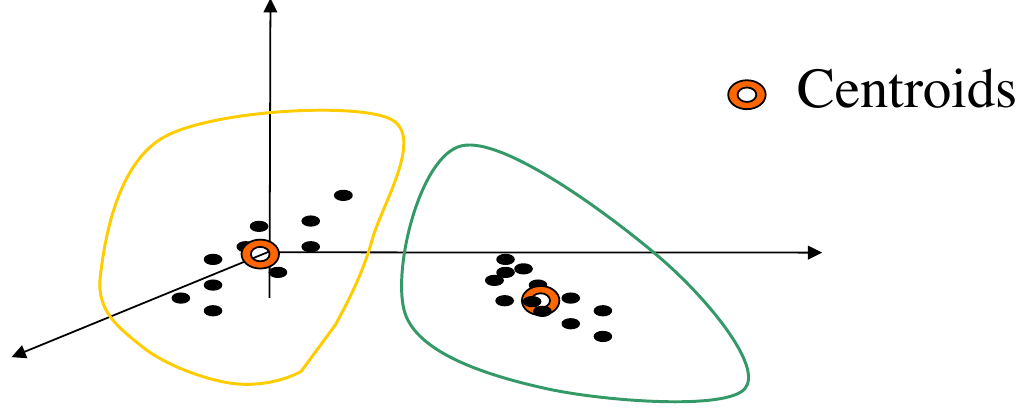
\includegraphics[width=0.54\linewidth,height=0.42\textheight,keepaspectratio]{images/03-l23_clustering.png}
\caption{Clustering: partizione dei dati in gruppi rappresentati da centroidi.}
\end{figure}

Il clustering è stato affrontato in moltissimi contesti e discipline,
con migliaia di algoritmi diversi: riflette la sua utilità come passo
dell'analisi esplorativa dei dati. Qui si adotta la prospettiva della
\textbf{quantizzazione vettoriale} per il \textbf{clustering
partizionale}.

\begin{boxwarning}{La metrica domina}

Come per il K-NN, è la \textbf{distanza assunta} a dire quali esempi
sono simili, e l'algoritmo decide i raggruppamenti in base a quella
metrica. La distanza euclidea è popolare ma è \textbf{solo una scelta},
e la scelta può avere implicazioni profonde (ad esempio si possono
pesare di meno gli outlier usando \(1 -\) una gaussiana centrata sul
prototipo).

\end{boxwarning}

\section{Quantizzazione vettoriale}\label{quantizzazione-vettoriale}

\begin{boxdefinition}{Vector Quantization (VQ)}

Le tecniche di quantizzazione vettoriale codificano una varietà di dati
\(V \subseteq \mathbb{R}^n\) usando solo un insieme finito
\(\mathbf{w} = (\mathbf{w}_1, \dots, \mathbf{w}_K)\) di vettori di
riferimento (\emph{codebook}) \(\mathbf{w}_i \in \mathbb{R}^n\). Un
vettore \(\mathbf{x} \in V\) è descritto dal vettore di riferimento
\textbf{vincente} (\emph{best matching})
\(\mathbf{w}_{i^*(\mathbf{x})}\), quello con distorsione
\(d(\mathbf{x}, \mathbf{w}_{i^*(\mathbf{x})})\) minima.

\end{boxdefinition}

Questo divide la varietà in sottoregioni, i \textbf{poliedri di
Voronoi}: \[
V_i = \{\mathbf{x} \in V \;:\; \|\mathbf{x} - \mathbf{w}_i\| \le \|\mathbf{x} - \mathbf{w}_j\| \;\forall j\},
\] e ogni \(\mathbf{x}\) è descritto dal vettore di riferimento
corrispondente.

\begin{figure}[htbp]
\centering
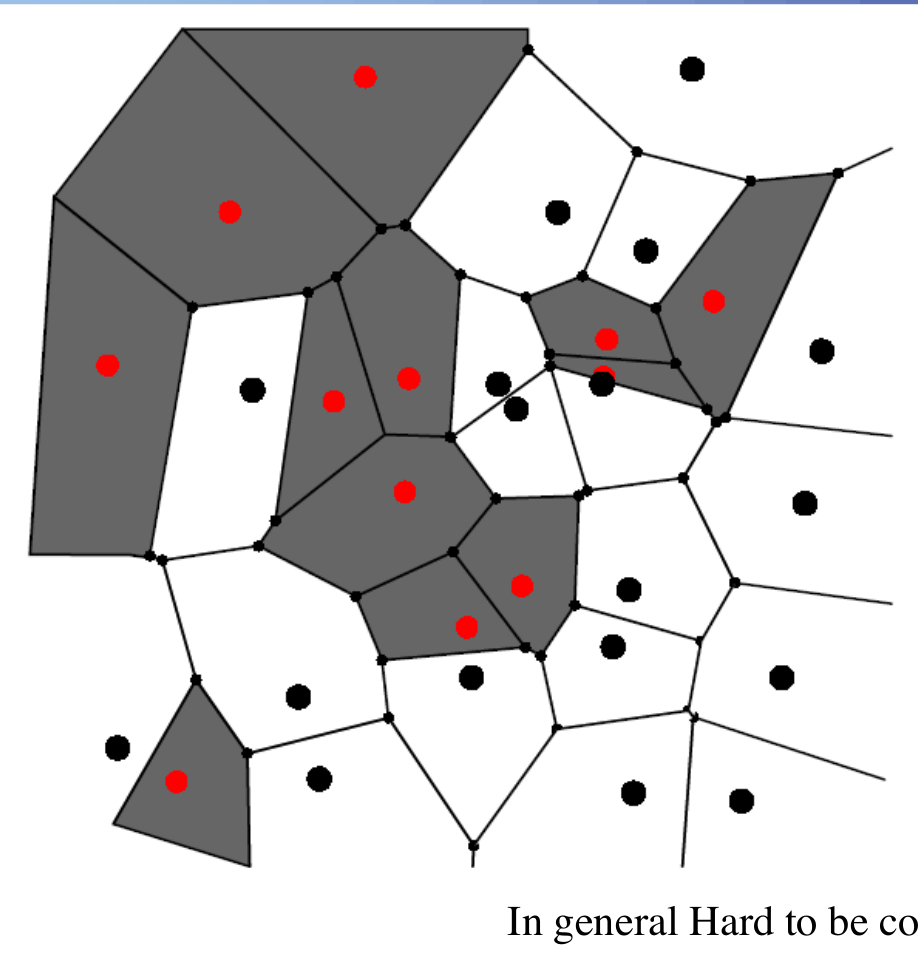
\includegraphics[width=0.43\linewidth,height=0.42\textheight,keepaspectratio]{images/19-som_voronoi.png}
\caption{Diagramma di Voronoi: ogni cella contiene i punti più vicini al suo
centro che a qualsiasi altro.}
\end{figure}

Il nostro problema è il contrario di quello del K-NN: \textbf{dato il
dataset, trovare i centri} che minimizzano la loss. In generale è
difficile: trovare il codebook ottimo è \textbf{NP-completo}.

\begin{boxexample}{Quantizzazione in 1D}

Nell'elaborazione digitale dei segnali, la \textbf{quantizzazione}
approssima un intervallo continuo di valori (o un insieme molto grande
di valori discreti) con un insieme relativamente piccolo di simboli
discreti, commettendo un errore di quantizzazione (distorsione). È ciò
che succede alla musica nei dispositivi digitali.

\begin{center}
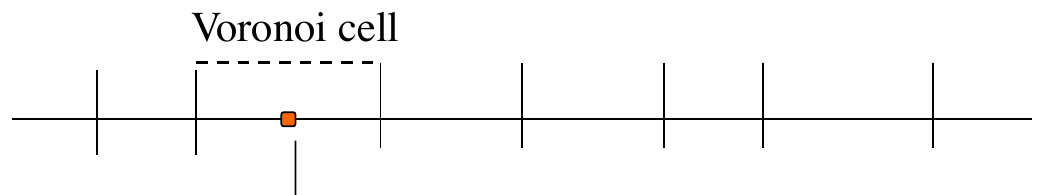
\includegraphics[width=0.54\linewidth,height=0.42\textheight,keepaspectratio]{images/19-som_quantizzazione-1d.png}
\end{center}

\end{boxexample}

\textbf{VQ e clustering.} Il clustering ha l'obiettivo più generale di
trovare raggruppamenti \textbf{interessanti o utili}, dove
``interessante'' è spesso definito implicitamente dalla procedura stessa
e non necessariamente dall'errore di quantizzazione minimo. Tuttavia la
VQ fornisce un quadro utile, e i suoi algoritmi sono spesso usati per il
clustering.

\subsection{L'errore di quantizzazione}\label{lerrore-di-quantizzazione}

L'obiettivo è partizionare in modo ottimo una distribuzione sconosciuta
nello spazio degli input in regioni approssimate da prototipi: un
insieme di quantizzatori
\(\mathbf{x} \mapsto c(\mathbf{x}) = \mathbf{w}_{i^*(\mathbf{x})}\), da
uno spazio continuo a uno discreto. Si considera la \textbf{distorsione
quadratica}
\(d(\mathbf{x}, c(\mathbf{x})) = \|\mathbf{x} - c(\mathbf{x})\|^2\); il
suo valore medio sulla distribuzione degli input è la distorsione (o
errore di ricostruzione, o di quantizzazione) attesa. \textbf{Questa è
la nostra loss}: \[
E = \int f\big(d(\mathbf{x}, \mathbf{w}_{i^*(\mathbf{x})})\big)\,p(\mathbf{x})\,d\mathbf{x} = \int \|\mathbf{x} - \mathbf{w}_{i^*(\mathbf{x})}\|^2\,p(\mathbf{x})\,d\mathbf{x},
\] dove \(p(\mathbf{x})\) è la distribuzione degli input. In versione
discreta, su \(l\) dati e \(K\) prototipi: \[
E = \sum_{i=1}^{l}\sum_{j=1}^{K}\|\mathbf{x}_i - \mathbf{w}_j\|^2\,\delta_{winner}(i, j), \qquad \delta_{winner}(i,j) = \begin{cases} 1 & \text{se } j \text{ è il vincitore per } \mathbf{x}_i \\ 0 & \text{altrimenti} \end{cases}
\] (\(\delta_{winner}\) è la funzione caratteristica del campo recettivo
di \(\mathbf{w}_j\)).

Minimizzare \(E\) rispetto a \(\mathbf{w}\) è il problema della VQ.
Attenzione: l'integrando \textbf{non è differenziabile con continuità},
perché il vincitore \(\mathbf{w}_{i^*(\mathbf{x})}\) cambia in modo
discreto al variare di \(\mathbf{x}\); si calcolano però le derivate
\textbf{localmente}, fissando \(\mathbf{x}\) in una cella di Voronoi.

\section{K-means}\label{k-means}

\subsection{Versione on-line}\label{versione-on-line}

Derivando \(E\) rispetto ai \(\mathbf{w}_j\) si ottiene la regola di
apprendimento della VQ, cioè il noto algoritmo \textbf{K-means} di Lloyd
e MacQueen (versione on-line): per ogni \(\mathbf{x}_i\), \[
\Delta\mathbf{w}_{i^*} = \eta\,\delta_{winner}(i, i^*)\,(\mathbf{x}_i - \mathbf{w}_{i^*}).
\] (La derivata di \(\|\mathbf{x}_i - \mathbf{w}_j\|^2\) rispetto a
\(\mathbf{w}_j\) è \(-2(\mathbf{x}_i - \mathbf{w}_j)\); muovendosi nel
verso opposto al gradiente si avvicina \(\mathbf{w}_j\) a
\(\mathbf{x}_i\).)

\begin{itemize}
\tightlist
\item
  Si modifica \textbf{solo il prototipo vincitore}, spostandolo verso
  \(\mathbf{x}\).
\item
  È una discesa del gradiente stocastica → \textbf{minimi locali}; il
  metodo dipende dall'\textbf{inizializzazione}.
\item
  Il \textbf{numero di cluster} va fornito in anticipo.
\end{itemize}

\subsection{Versione batch}\label{versione-batch}

\begin{boxabstract}{Algoritmo K-means batch (Linde-Buzo-Gray, o Lloyd generalizzato)}

\begin{enumerate}
\def\labelenumi{\arabic{enumi}.}
\tightlist
\item
  Scegliere \(K\) centri: \(K\) pattern estratti a caso, o \(K\) punti
  casuali nell'ipervolume che contiene i pattern.
\item
  Assegnare ogni pattern al centro più vicino (il \textbf{vincitore}):
  \[
  i^*(\mathbf{x}) = \arg\min_i \|\mathbf{x} - \mathbf{w}_i\|^2, \qquad \|\mathbf{x} - \mathbf{w}_i\|^2 = \sum_{j=1}^{n}(x_j - w_{ij})^2.
  \]
\item
  Ricalcolare i centri come \textbf{media} (centroide geometrico) dei
  membri del cluster: \[
  \mathbf{w}_i = \frac{1}{|\text{cluster}_i|}\sum_{\mathbf{x}_j \in \text{cluster}_i}\mathbf{x}_j.
  \]
\item
  Se il criterio di convergenza non è soddisfatto (nessuna o minima
  riassegnazione dei pattern, minima diminuzione dell'errore
  quadratico), tornare al passo 2.
\end{enumerate}

\end{boxabstract}

(Esercizio: dalla versione on-line a quella batch. Sommando --- o
mediando --- sui pattern di un cluster il delta on-line con
\(\eta = 1\), si ottiene
\(\mathbf{w}_{new} = \mathbf{w}_{old} + \frac{1}{|C|}\sum_{\mathbf{x} \in C}(\mathbf{x} - \mathbf{w}_{old}) = \frac{1}{|C|}\sum_{\mathbf{x} \in C}\mathbf{x}\):
proprio la media.)

\begin{figure}[htbp]
\centering
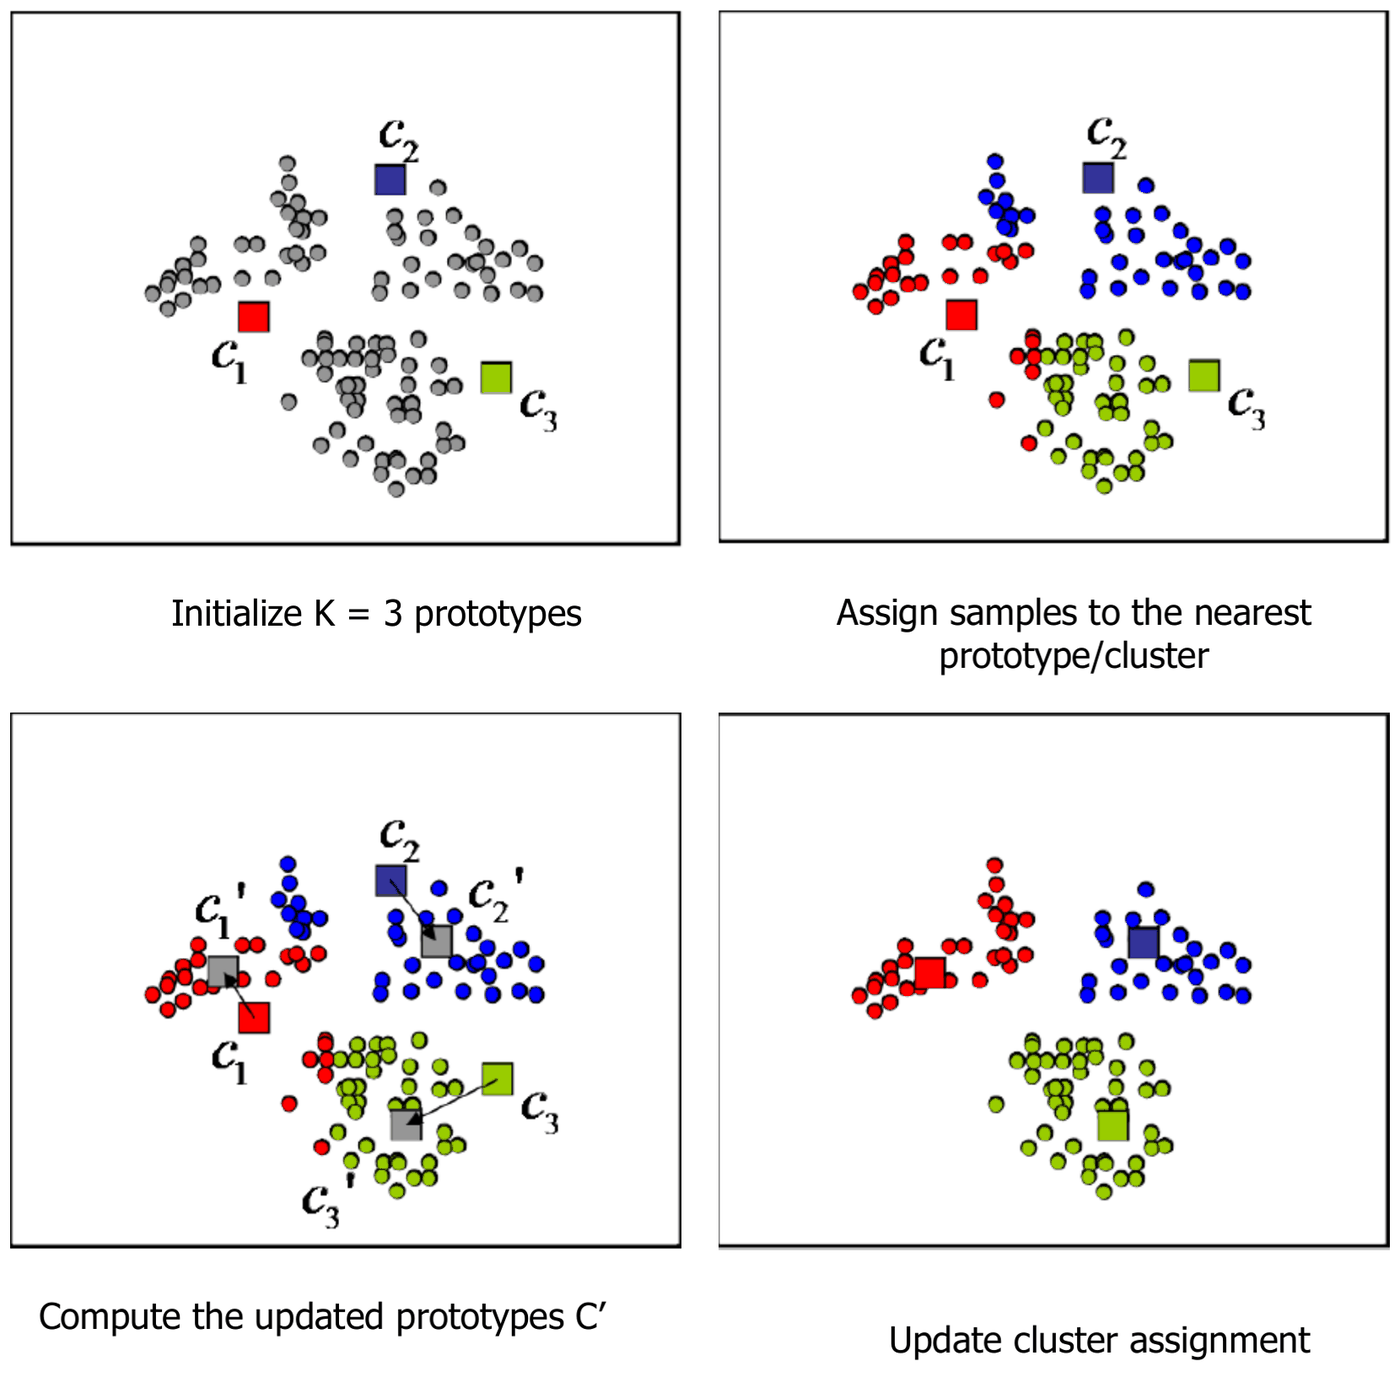
\includegraphics[width=0.80\linewidth,height=0.42\textheight,keepaspectratio]{images/19-som_kmeans.png}
\caption{Esempio di K-means con \(K = 3\): inizializzazione, assegnazione,
aggiornamento dei prototipi, nuova assegnazione.}
\end{figure}

\subsection{Pregi e difetti}\label{pregi-e-difetti}

\begin{itemize}
\tightlist
\item
  È l'algoritmo più semplice e usato con un criterio d'errore
  quadratico; è popolare perché facile da implementare e in generale
  efficiente.
\item
  Il numero \(K\) di cluster va fornito.
\item
  I minimi locali di \(E\) rendono il metodo dipendente
  dall'inizializzazione, con scelte solo sub-ottime dei prototipi.
\item
  Funziona molto bene per cluster \textbf{compatti e ipersferici}; con
  cluster di altre forme (ad esempio due ``spirali'' intrecciate)
  fallisce.
\item
  \textbf{Nessuna proprietà di visualizzazione}: non permette di
  proiettare i dati in uno spazio a dimensione minore, e
  l'indicizzazione dei \(\mathbf{w}\) è arbitraria, quindi la mappatura
  non è ordinata.
\end{itemize}

\subsection{Soft-max}\label{soft-max}

Per evitare i minimi locali si introduce una regola di adattamento
\textbf{soft-max}: non si modifica solo il vincitore, ma \textbf{tutti}
i centri, in base alla loro \textbf{vicinanza} a \(\mathbf{x}\), con un
passo che decresce con la distanza \(d(\mathbf{x}, \mathbf{w}_i)\) (ad
esempio il \emph{maximum-entropy clustering} con distanze gaussiane).
Un'istanza di questa strategia nelle reti neurali sono le \textbf{SOM di
Kohonen}, dove però la vicinanza tra i vettori di riferimento è definita
su una \textbf{mappa ordinata}, cioè una griglia neurale su cui sono
disposti.

\section{Self-Organizing Map}\label{self-organizing-map}

Le \textbf{Self-Organizing Map} (SOM), o \textbf{mappe di Kohonen}
(1981), sono reti di \(N\) neuroni disposti su una \textbf{griglia
regolare a bassa dimensione} (di solito 2D, un \emph{lattice}).

\begin{itemize}
\tightlist
\item
  Ogni unità è identificata dalle sue \textbf{coordinate} sulla mappa.
\item
  Ogni unità riceve \textbf{lo stesso input} \(\mathbf{x}\).
\item
  Ogni unità ha un \textbf{peso} \(\mathbf{w}\), con
  \(\dim(\mathbf{w}) = \dim(\mathbf{x}) = n\).
\end{itemize}

\subsection{Obiettivo}\label{obiettivo}

La SOM impara una mappa dallo spazio degli input a un reticolo di unità
neurali che \textbf{preserva la topologia}:

\begin{itemize}
\tightlist
\item
  unità vicine sulla mappa rispondono a pattern di input simili;
\item
  punti vicini nello spazio di input vengono mappati sulla stessa unità
  o su unità vicine;
\item
  la mappa di output (2D) ha proprietà di \textbf{visualizzazione}.
\end{itemize}

\begin{figure}[htbp]
\centering
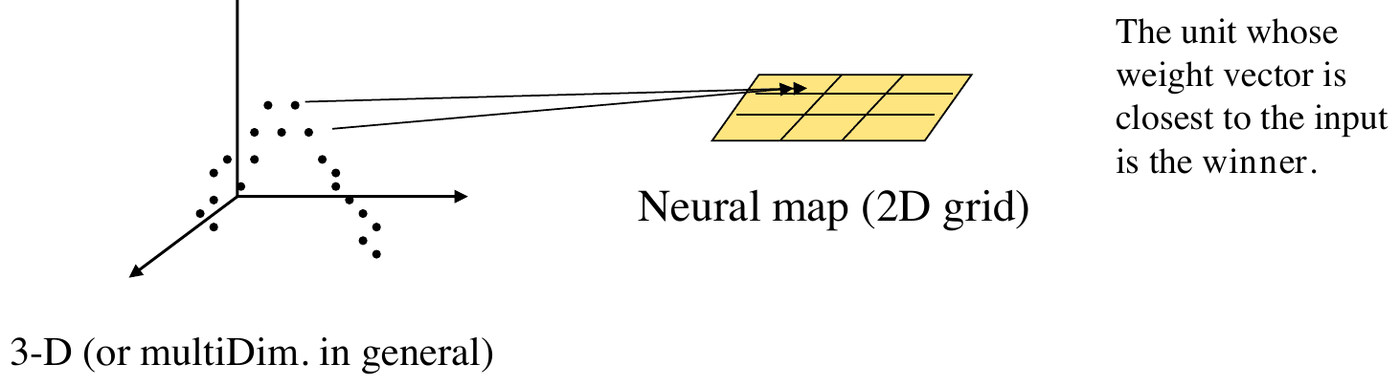
\includegraphics[width=0.74\linewidth,height=0.42\textheight,keepaspectratio]{images/19-som_mappa.png}
\caption{Una SOM mappa lo spazio di input (qui 3D) su una griglia neurale 2D.}
\end{figure}

Usi della SOM:

\begin{itemize}
\tightlist
\item
  \textbf{clustering}: i cluster si identificano sulla mappa (si trovano
  rapidamente strutture nei dati);
\item
  \textbf{pattern recognition e VQ}: l'input viene trasformato nel
  vettore dei pesi del neurone più vicino (il vettore del codebook);
\item
  \textbf{compressione}: l'input viene trasformato nell'indice (codice)
  dell'unità vincitrice;
\item
  \textbf{proiezione ed esplorazione}: la distribuzione dei dati
  multidimensionali si visualizza in uno spazio a dimensione minore (la
  mappa 2D).
\end{itemize}

\subsection{Apprendimento competitivo e ispirazione
biologica}\label{apprendimento-competitivo-e-ispirazione-biologica}

L'\textbf{apprendimento competitivo} è un processo adattivo in cui i
neuroni diventano gradualmente sensibili (specializzati) a categorie o
insiemi di input diversi: i neuroni \textbf{competono} per un dato, e il
vincitore apprende di più.

La natura sfrutta questo meccanismo: nella \textbf{corteccia
somatosensoriale} (e motoria) c'è una mappa \textbf{topologicamente
ordinata} del corpo, l'\textbf{homunculus}. Neuroni adiacenti
rappresentano sorgenti di attivazione vicine nel corpo, e le parti più
sensibili occupano aree più ampie della corteccia. In una mappa che
preserva la topologia, unità fisicamente vicine rispondono a classi di
input a loro volta vicine.

\begin{figure}[htbp]
\centering
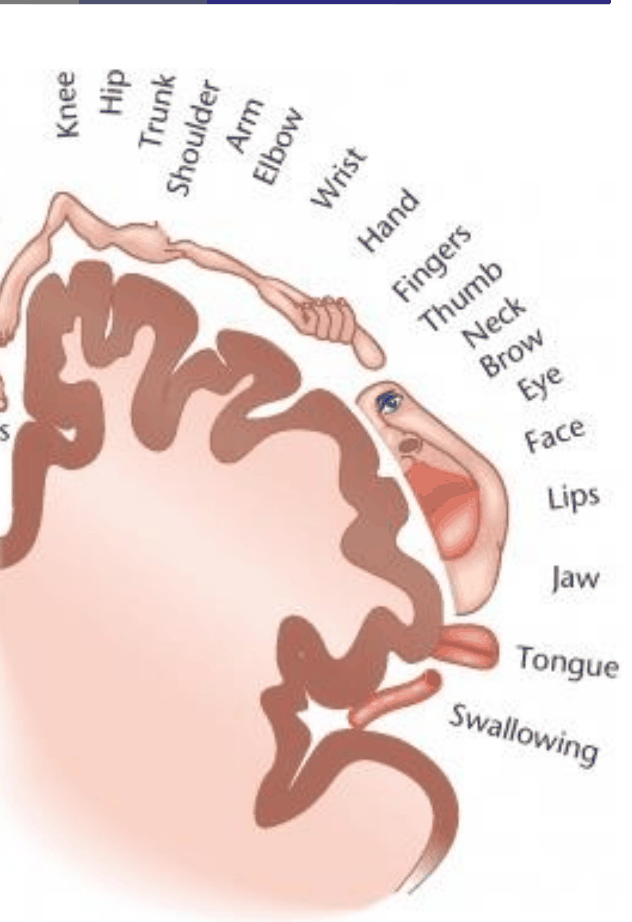
\includegraphics[width=0.31\linewidth,height=0.42\textheight,keepaspectratio]{images/19-som_homunculus.png}
\caption{L'homunculus: una mappa topologicamente ordinata del corpo nella
corteccia.}
\end{figure}

\subsection{L'algoritmo}\label{lalgoritmo}

\begin{boxabstract}{Algoritmo SOM}

\begin{itemize}
\tightlist
\item
  Inizializzare casualmente i pesi della mappa.
\item
  Estrarre un input \(\mathbf{x}\).
\item
  \textbf{Fase competitiva}: il vincitore è l'unità con \(\mathbf{w}\)
  più simile a \(\mathbf{x}\).
\item
  \textbf{Fase cooperativa}: aggiornare i pesi delle unità che hanno
  relazioni topologiche \textbf{sulla mappa} con il vincitore (una forma
  di soft-max).
\item
  Continuare fino a convergenza (nessun cambiamento).
\end{itemize}

\textbf{Fattore chiave}: i vicini \textbf{sulla mappa} (mentre il
soft-max standard usa la vicinanza nello spazio dei dati).

\end{boxabstract}

\subsubsection{Fase competitiva}\label{fase-competitiva}

L'input \(\mathbf{x}\) viene confrontato con i pesi di tutte le unità
con la distanza euclidea. La SOM standard adotta una strategia
\textbf{winner-take-all} (come il K-means): \[
i^*(\mathbf{x}) = \arg\min_i \|\mathbf{x} - \mathbf{w}_i\|,
\] dove \(i\) è un indice sulla mappa (ad esempio le coordinate 2D).

\subsubsection{Fase cooperativa}\label{fase-cooperativa}

I pesi del vincitore \textbf{e delle unità del suo vicinato} vengono
avvicinati all'input (apprendimento hebbiano). All'iterazione \(t\): \[
\mathbf{w}_i(t+1) = \mathbf{w}_i(t) + \eta(t)\,h_{i,i^*(\mathbf{x})}(t)\,\big[\mathbf{x} - \mathbf{w}_i(t)\big],
\] dove \(h\) è la \textbf{funzione di vicinato} (\emph{neighborhood
kernel}), che decresce monotonamente all'aumentare della distanza
\textbf{sulla mappa} tra l'unità \(i\) e il vincitore. Ad esempio una
gaussiana: \[
h_{i,i^*}(t) = \exp\left(-\frac{\|\mathbf{r}_i - \mathbf{r}_{i^*}\|^2}{2\sigma^2(t)}\right),
\] con \(\mathbf{r}_i\) le coordinate dell'unità \(i\) sulla griglia e
\(\sigma(t)\) la larghezza.

Il \textbf{learning rate} \(\eta\) e il \textbf{raggio del vicinato}
\(\sigma\) diminuiscono con le iterazioni: il vicinato è \textbf{ampio
all'inizio} (ordinamento globale della mappa) e poi si restringe
lentamente durante l'apprendimento (convergenza, raffinamento locale).
In pratica la forma del vicinato si sceglie tra forme geometriche
standard sulla griglia (rettangolare, esagonale\ldots) che includono un
insieme finito di unità.

\subsection{L'emergere dell'ordine
topologico}\label{lemergere-dellordine-topologico}

La regola della fase cooperativa è \textbf{fondamentale} per la
formazione di mappe topograficamente ordinate. I pesi non vengono
modificati indipendentemente, ma \textbf{per sottoinsiemi
topologicamente legati}: a ogni passo si seleziona il vicinato del
vincitore sulla griglia, e tutte le unità del sottoinsieme ricevono
aggiornamenti simili. Così l'informazione topologica viene trasmessa
alla mappa: il vincitore e i suoi vicini sulla griglia ricevono
aggiornamenti simili e, dopo l'apprendimento, rispondono a input simili.
Anche se sembra naturale, una dimostrazione formale dell'ordinamento è
difficile.

\begin{boxtip}{K-means contro SOM}

\begin{itemize}
\tightlist
\item
  \textbf{K-means}: aggiorna solo il vincitore; i prototipi non hanno
  alcun ordine; non c'è visualizzazione.
\item
  \textbf{SOM}: aggiorna il vincitore \textbf{e i suoi vicini sulla
  griglia}, con un vicinato che si restringe nel tempo; i prototipi sono
  disposti su una mappa ordinata che \textbf{preserva la topologia},
  permettendo la visualizzazione; il vicinato ampio iniziale aiuta anche
  a evitare i minimi locali. (Con vicinato di raggio zero, la SOM si
  riduce al K-means on-line.)
\end{itemize}

\end{boxtip}

\begin{figure}[htbp]
\centering
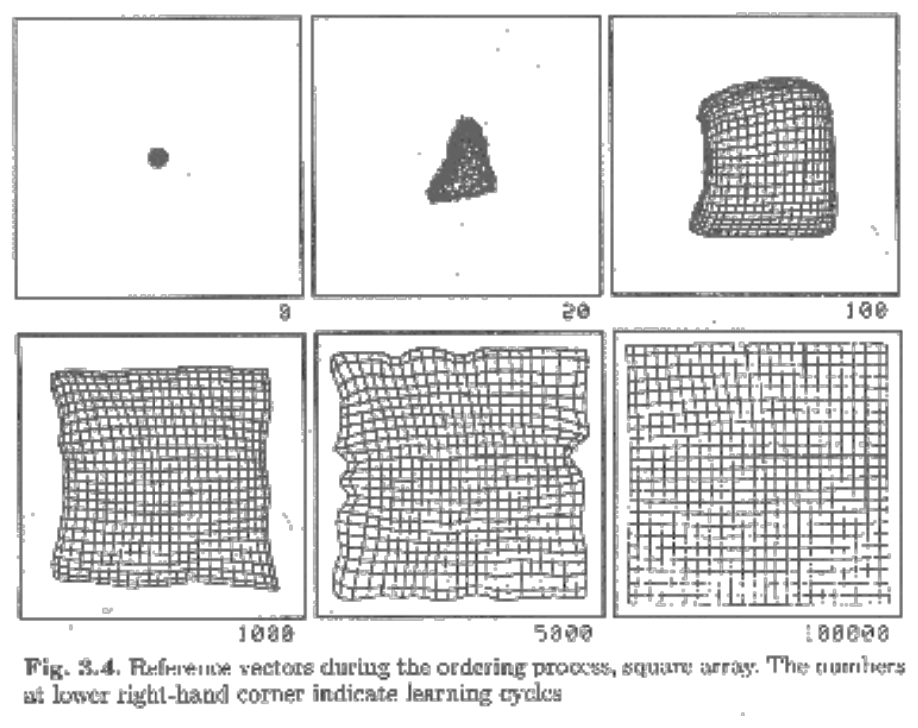
\includegraphics[width=0.69\linewidth,height=0.42\textheight,keepaspectratio]{images/19-som_training-uniforme.png}
\caption{Addestramento di una SOM su dati uniformi in 2D: i vettori di
riferimento (collegati secondo la griglia) si distendono
progressivamente sulla distribuzione.}
\end{figure}

Durante l'addestramento le unità ``vanno a rappresentare'' i cluster dei
dati.

\subsection{Visualizzazione}\label{visualizzazione}

La mappa si può usare per visualizzare diverse caratteristiche della SOM
e dei dati:

\begin{itemize}
\tightlist
\item
  la \textbf{densità} dei vettori di riferimento (colore proporzionale
  al numero di ``hit'');
\item
  le \textbf{distanze} tra i prototipi di unità vicine
  (\textbf{U-matrix}): colori scuri indicano grandi distanze tra unità
  adiacenti, colori chiari piccole distanze;
\item
  le mappe di Sammon (con linee)\ldots{}
\end{itemize}

Questo rende la SOM facilmente \textbf{interpretabile}.

\begin{boxexample}{Welfare e povertà nel mondo (Kaski e Kohonen, 1995)}

39 indicatori di benessere per 77 paesi (World Development Report 1992).
Sulla mappa 13×9, il grigio tra due unità indica la distanza (scalata e
smussata) tra i loro vettori di riferimento: le zone chiare sono cluster
di paesi simili, le zone scure i confini tra cluster. Non serve alcuna
ipotesi a priori sulla forma dei cluster.

\begin{center}
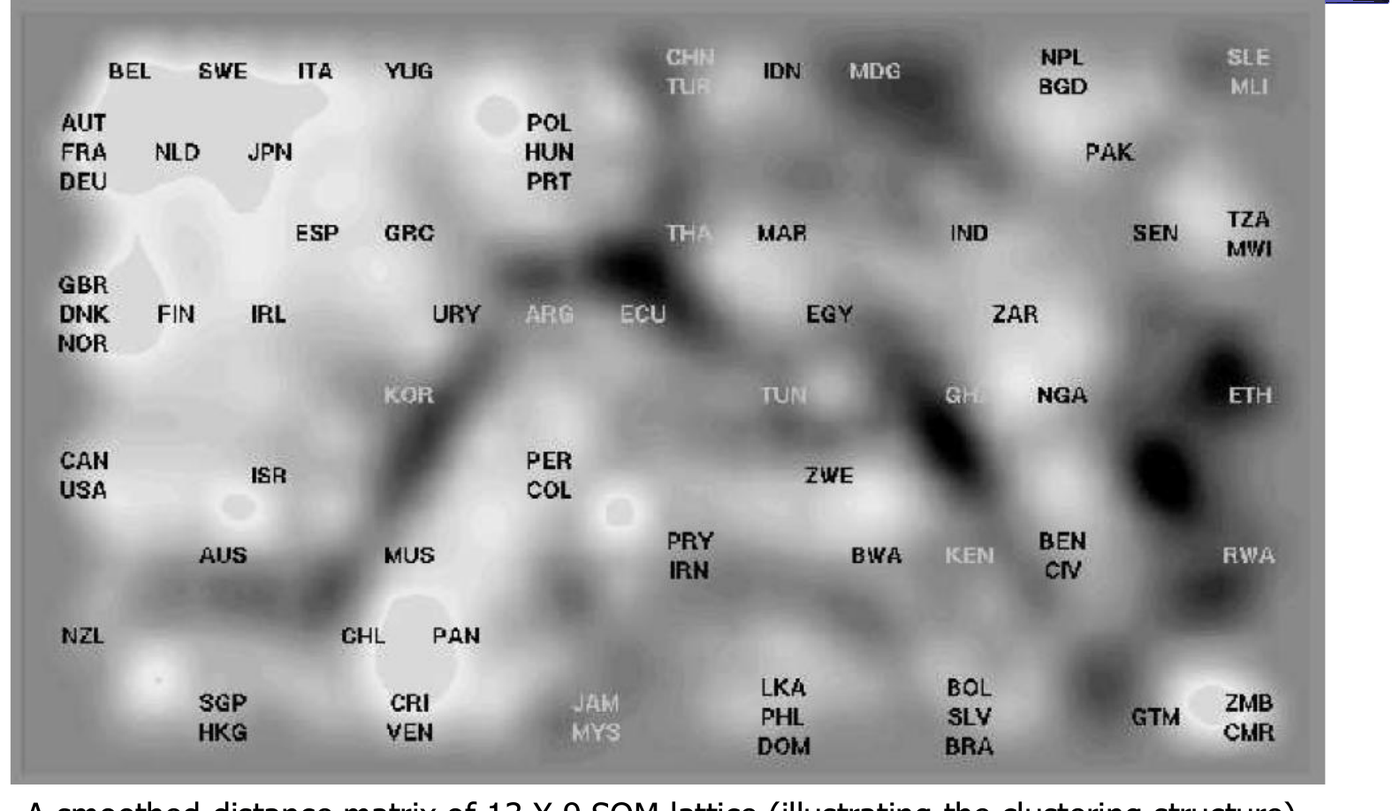
\includegraphics[width=0.80\linewidth,height=0.42\textheight,keepaspectratio]{images/19-som_umatrix.png}
\end{center}

\begin{center}
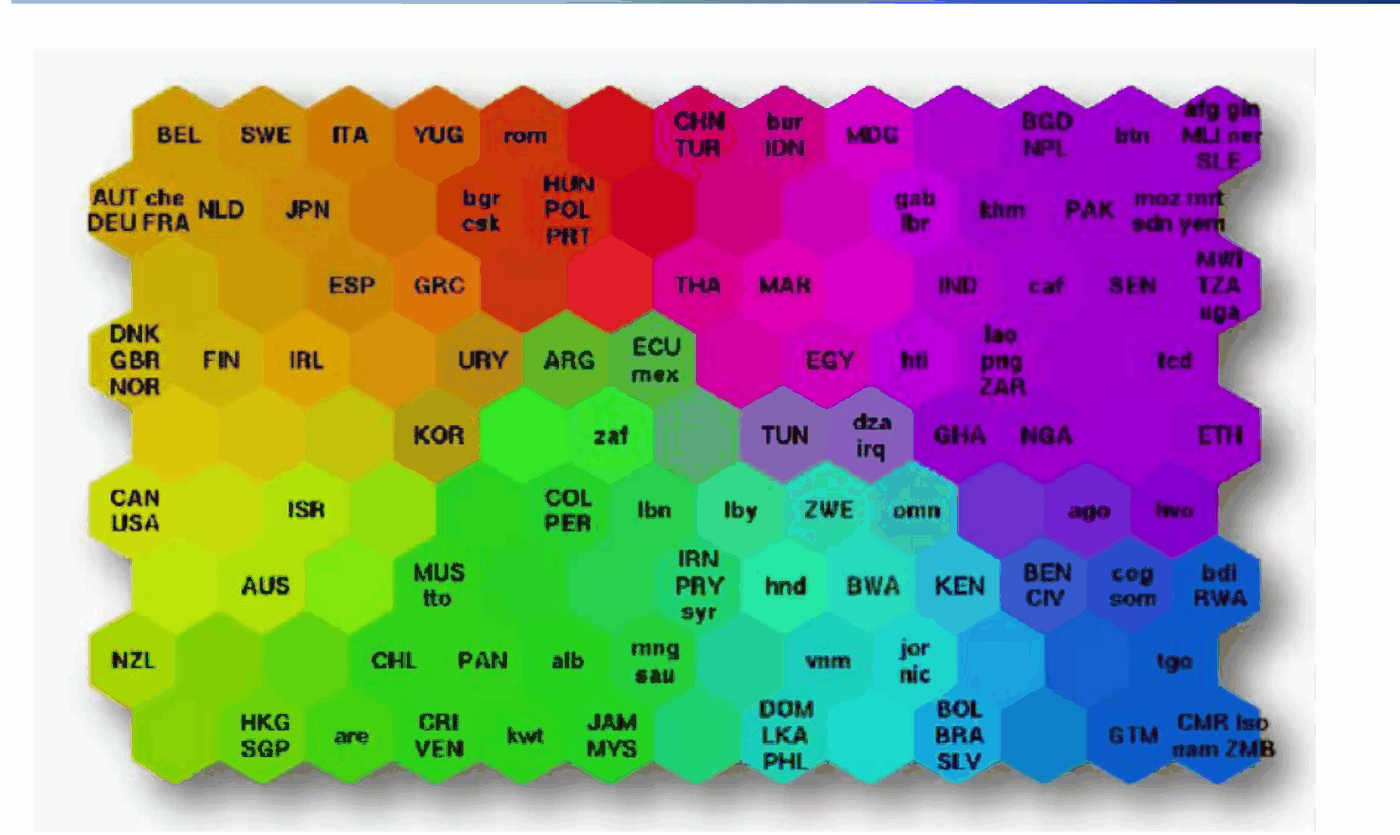
\includegraphics[width=0.80\linewidth,height=0.42\textheight,keepaspectratio]{images/19-som_mappa-colori.png}
\end{center}

\end{boxexample}

\section{Valutare un clustering
(cenni)}\label{valutare-un-clustering-cenni}

Come si valuta il risultato di un clustering? Cosa distingue un
risultato buono da uno scadente?

\begin{itemize}
\tightlist
\item
  La valutazione è spesso \textbf{soggettiva}: esistono pochi ``gold
  standard'', tranne in sotto-domini ben definiti.
\item
  Misure \textbf{oggettive}, come l'errore di quantizzazione (che però
  dipende dal numero di centroidi).
\item
  \textbf{Non} si usa banalmente l'etichetta di un task di
  classificazione sottostante (la \emph{purity}, con entropia,
  informazione mutua\ldots): se si hanno le etichette, tanto vale usare
  un classificatore.
\item
  Qualità del modello/clustering contro qualità dei risultati
  (dipendente dal dominio).
\end{itemize}

Altri argomenti dell'apprendimento non supervisionato: clustering
gerarchico (dendrogrammi), analisi delle componenti principali (e di
curve e superfici principali), regole di associazione, ICA,
Multidimensional Scaling, t-SNE, Generative Topographic Mapping, reti
ART.

\begin{boxquestion}{Possibili domande d'esame}

\begin{itemize}
\tightlist
\item
  Definire clustering e quantizzazione vettoriale. Cos'è l'errore di
  quantizzazione?
\item
  Derivare la regola on-line del K-means e passare alla versione batch.
\item
  Pregi e difetti del K-means.
\item
  Descrivere la SOM: architettura, fase competitiva, fase cooperativa,
  funzione di vicinato.
\item
  Perché la SOM preserva la topologia? Differenze tra K-means e SOM.
\item
  Come si visualizza una SOM (U-matrix)?
\end{itemize}

\end{boxquestion}
